\chapter*{Wstęp}
\addcontentsline{toc}{chapter}{Wstęp}
\section*{Wprowadzenie}
Analiza metryk jest ważnym aspektem prowadzenia projektów informatycznych. Pozwalają one na wgląd do wielu parametrów projektu i na tej podstawie podejmowanie ważnych decyzji związanych z jego prowadzeniem.
Nauka tej analizy nie jest prostym zadaniem -- dostęp do danych realistycznych projektów na potrzeby szkoleń jest bardzo ograniczony, często z uwagi na poufne dane. Ponadto, nie istnieją rozwiązania pozwalające na przeprowadzanie
symulacji projektów do celów dydaktycznych na najpopularniejszych platformach.

Praca "Generowanie danych na potrzeby nauki metryk w inżynierii oprogramowania" podejmuje analizę różnych metryk w inżynierii oprogramowania oraz platform do zarządzania projektami pod kątem możliwości automatyzacji tego procesu,
oraz proponuje rozwiązanie tego problemu, poprzez opracowanie narzędzia umożliwiającego symulacje projektów informatycznych na platformach
będących w powszechnym użytku komercyjnym.

Nauka analizy metryk jest również elementem zajęć na uczelni, a więc istnieje środowisko w którym można szybko przetestować narzędzie w praktyce i trwale udoskonalać.

\section{Cel pracy}
Celem pracy jest opracowanie automatyzacji wspomnianego we wstępie pracy procesu przygotowywania materiałów do zajęć.
W ramach projektu powstała aplikacja umożliwiająca generowanie projektów w metodyce Kanban na wybranej platformie.
Program umożliwia zdefiniowanie parametrów:
\begin{itemize}
    \item Nazwa projektu
    \item Autor projektu
    \item Data rozpoczęcia projektu
    \item Data zakończenia projektu
    \item Ilość zadań w projekcie
\end{itemize}

\section*{Plan Pracy}
W pierwszym rodziale pracy ma miejsce przegląd różnych metryk w inżynierii oprogramowania, pod kątem ich przydatności w pomiarze pracy zespołu.
Porównywane są tutaj metryki statyczne oraz metryki z metodyk zwinnych Scrum i Kanban.

Drugi rozdział opisuje przegląd platform służących do zarządzania projektami, dokładniejszą analizę funkcjonalności wybranych z nich.
Na końcu rozdziału dokonany i uzasadniony jest wybór platformy do realizacji rozwiązania.

W trzecim rozdziale opisana jest implementacja oraz weryfikacja rozwiązania.

Ostatni rozdział podsumowuje pracę -- jakie cele udało się osiągnąć, jakich udoskonaleń względem zakresu pracy nie udało się zaimplementować, oraz
omawia możliwości dalszego rozwoju projektu.


\chapter{Metryki w Inżynierii Oprogramowania}
\section{Metryki Statyczne}
Pierwszym rodzajem omawianych metryk są metryki statyczne. Spośród omawianych w tej pracy metryk wyróżniają się tym,
że jako jedyne nie skupiają się na mierzeniu parametrów pracy zespołu, tylko kodu.
Część z nich jest w dzisiejszych czasach zintegrowana w narzędziach deweloperskich, takich jak \href{https://www.synopsys.com/software-integrity/static-analysis-tools-sast/coverity.html}{Coverity}
lub \href{https://www.sonarsource.com/products/sonarlint/}{SonarLint}.

\subsection{Liczba linii kodu}
\label{loc}
Najprostszą metryką statyczną jest liczba linii kodu (ang. Lines of Code, LOC). Liczba linii kodu nie bierze pod uwagę pustych linii oraz komentarzy.

Aby przełożyć ją na metrykę mierzącą pracę zespołu, można mierzyć LOC na dany okres.

Jest to dobra metryka do orientacyjnej oceny rozmiaru projektu czy danej funkcjonalności, jednak nie nadaje
się do dokładniejszych analiz, ze względu na fundamentalne wady.

\subsubsection*{Mniej linii nie zawsze oznacza lepszy kod}
Jako przykład można przyjrzeć się tzw. \textit{fluent API}, czyli interfejsom programistycznym zaprojektowanym z myślą o łańcuchowym wywoływaniu metod.

Przykładem takich interfejsów są np. Stream API, AssertJ, czy JOOQ (Java).
Przy korzystaniu z tego typu interfejsów, wywoływanie kolejnych metod w pojedynczej linii jest bardzo nieczytelne, zalecane jest
umieszczanie każdego wywołania metody w nowej linii, co wpływa negatywnie na metrykę LOC.
\begin{lstlisting}[caption=Sumowanie liczb pierwszych przy użyciu Stream API (Java)]
var primesSum = IntStream.range(1, 1_000)
    .filter(SomeLibrary::isPrime)
    .sum();
\end{lstlisting}

\newpage
\subsubsection*{Różnice składni i stylu kodu}
Niektóre języki mają po prostu bardziej zwięzłą składnię niż inne.

Przykładowo, JavaScript i Kotlin posiadają operator \texttt{?}, pozwalający pisać w 1 linii kod, który w Javie zająłby 4:
\begin{lstlisting}[caption=Przykład obsługi null (Kotlin)]
val obj = a?.field;
\end{lstlisting}
\begin{lstlisting}[caption=Przykład obsługi null (Java)]
Object obj = null;
if (a != null) {
    obj = a.field;
}
\end{lstlisting}

\subsubsection*{Refaktoryzacja}
Istotnym elementem utrzymywania dobrej jakości kodu w dużych projektach informatycznych jest refaktoryzacja, czyli niefunkcjonalne zmiany nie niosące stricte dodatkowej wartości biznesowej,
a jedynie polepszające jakość kodu w celu ułatwienia jego utrzymania w przyszłości.

Częstym elementem refaktoryzacji jest usuwanie tzw. \textit{martwego kodu}, czyli kodu który nie jest wykorzystywany -- np. gałęzie wyrażeń \texttt{switch} czy \texttt{if} które są nieosiągalne, nieużywanych metod, zmiennych czy testów.
Innym elementem refaktoryzacji bardzo często jest skracanie istniejącego kodu do bardziej czytelnej formy.

W przypadku mierzenia LOC na okres do analizy pracy, w przypadku refaktoryzacji ta metryka może fałszywie wskazać ujemną wydajność zespołu.

\subsection{Metryki Halsteada}
W 1977 prof Maurice Howard Halstead z Purdue University, sformułował metryki mające opisywać kod w dokładny sposób.\cite{halstead1977elements}
Metryki prof Halsteada opierają się o 4 wartości:
\begin{itemize}
    \item $\eta_1$ -- liczba unikalnych operatorów
    \item $\eta_2$ -- liczba unikalnych operandów
    \item $N_1$ -- całkowita liczba operatorów
    \item $N_2$ -- całkowita liczba operandów
\end{itemize}
Na ich podstawie można obliczyć następujące parametry:
\begin{itemize}
    \item Słownictwo: $\eta = \eta_1 + \eta_2$
    \item Długość: $N = N_1 + N_2$
    \item Szacunkowa długość: $\hat{N} = \eta_1log_2\eta_1 + \eta_2log_2\eta_2$
    \item Objętość: $V = N \times log_2\eta$
    \item Trudność: $D = \frac{\eta_1}{2} \times \frac{N_2}{\eta_2}$
    \item Wysiłek: $E = D \times V$
    \item Czas: $T = \frac{E}{18}[s]$
    \item Bugi: $B = \frac{E^{\frac{2}{3}}}{3000}$ Później uproszczone do $B = \frac{V}{3000}$
\end{itemize}
\newpage
Metryki te nie przyjęły się, ze względu na ich właściwości:
\begin{enumerate}
    \item Objętość programu jest liniowo zależna od długości
    \item Wysiłek jest liniowo zależny od objętości
    \item Czas jest liniowo zależny od wysiłku
\end{enumerate}
Łańcuch tych zależności sprowadza się do tego, że każda z tych metryk jest u podstaw liniowo zależna od długości, która pod kątem przydatności niewiele różni się od liczby linii kodu.

Zebranie odpowiednich parametrów kodu i obliczenie tych metryk jest zatem inwestycją czasu, która w porównaniu z LOC jest nieopłacalna.

\subsection{Złożoność cyklomatyczna i kognitywna}
Złożoność cyklomatyczna to metryka służąca do oceny złożoności programów, ze szczególnym uwzględnieniem ich struktury sterowania. Wprowadził ją w 1976 roku Thomas McCabe jako narzędzie do mierzenia
liczby niezależnych ścieżek w kodzie źródłowym. \cite[]{ComplexityMeasure}

Często zapisywana jako $V(G)$, jest definiowana jako liczba niezależnych ścieżek w grafie przepływu sterowania programu.

Można obliczyć ją na podstawie struktury grafu przepływu sterowania:
$V(G) = E - N + 2P$,
gdzie:
\begin{itemize}
    \item $E$ - liczba krawędzi w grafie
    \item $N$ - liczba węzłów w grafie
    \item $P$ - liczba połączonych komponentów grafu
\end{itemize}
Albo na podstawie liczby decyzji:
$V(G) = D + 1$,
gdzie:
\begin{itemize}
    \item $D$ - liczba węzłów decyzyjnych w grafie przepływu sterowania (instrukcje \texttt{if}, \texttt{switch}, pętle)
\end{itemize}
Złożoność cyklomatyczna nadaje się jednak do stosowania jedynie na poziomie pojedynczych metod oraz nie uwzględnia złożonych warunków logicznych.

Ze względu na to że złożoność powstała w czasach mniej zaawansowanych języków programowania, obecnie w jej miejsce stosowana jest złożoność kognitywna. \cite[]{CognitiveComplexity}
Złożoność kognitywna bierze pod uwagę również struktury związane z nowymi językami programowania, jak np. bloki \texttt{try/catch} czy wyrażenia lambda.

Złożoność kognitywna jest bardzo dobrą metryką w procesie tworzenia oprogramowania. Pozwala na ocenę trudności testowania danych modułów lub monitorowanie kiedy już czas na refaktoryzację, ponieważ złożoność za bardzo urosła.

Metryka ta nie nadaje się jednak zupełnie do pomiaru pracy, jako że skupia się w całości na poziomie skomplikowania kodu źródłowego.

\section{Metryki w metodyce Scrum}
Chociaż oficjalny Scrum Guide \cite{Schwaber2012TheSG} nie definiuje bezpośrednio metryk, powszechnie przyjęło się korzystanie z \textit{Velocity} oraz wykresów wypalenia.

\subsection{Czym są Story Points?}
Mimo że Scrum jest nieco starszy niż Extreme Programming, koncepcja Story Points została zaczerpnięta właśnie z XP.
Na swoim blogu \cite{StoryPointsRevisited} jeden z autorów tej metodyki opisuje że początkowo estymaty ustalało się po prostu w liczbie dni.
Nie była to jednak najbardziej precyzyjna jednostka do estymacji, a więc szybko został zaadaptowany koncept tzw. \textit{Dni Idealnych}.
Ron Jeffries opisuje dni idealne następującymi słowami: \textit{"We quickly went to what we called “Ideal Days”, which was informally described as how long it would take a pair to do it if the bastards would just leave you alone."}.
Kolokwialnie mówiąc, dni idealne to dni w których programiści mieliby święty spokój.
Aby z liczby dni idealnych uzyskać estymatę faktycznego czasu, były one mnożone przez współczynnik obciążenia.
Nazwa "dni idealne" często była skracana do "dni", co prowadziło do nieporozumień z klientami, stąd zaczęto nazywać je po prostu "punktami". \\
Obecnie Story Points funkcjonują jako relatywna jednostka, nie mająca bezpośredniego przełożenia na czas wykonania, a używana jedynie do oceny ilości pracy.

\subsection{Velocity}
Velocity jest bardzo prostą metryką, polegającą jedynie na zsumowaniu wagi zadań w danym sprincie, dając wgląd w wydajność zespołu.
Metryka ta niestety jest bardzo podatna na niepoprawne estymowanie zadań -- świadomie bądź nie, co może prowadzić do fałszywej oceny postępów w przypadku
zespołów które jeszcze się nie "skalibrowały" i niedoestymowują zadań, oraz zespołów które celowo je przeestymowują aby wypaść lepiej na papierze.

\subsection{Wykres wypalenia}
Błędnie nazywany metryką, ponieważ jest to jedynie wizualizacja postępu projektu.
Oś Y reprezentuje skumulowaną wagę pozostałych zadań, natomiast oś X czas.
Na wykresie wypalenia można zidentyfikować czy zespół nadąża z wykonywaniem zadań.
W dobrze przebiegającym projekcie powinien być obserwowalny trend spadkowy, moment kiedy wartość na osi Y spadnie do 0 jest momentem wykonania wszystkich zadań na zadany okres.

\subsection{Inne Metryki}
Jako że metryki nie są oficjalnie zdefiniowane, zależą one tak naprawdę od organizacji.
Firmy zajmujące się wspieraniem produkcji oprogramowania (np. \href{https://www.atlassian.com/}{Atlassian}, \href{https://www.sealights.io/}{Sealights}), wymieniają tutaj m.in. \cite{ScrumMetricsSealights} \cite{ScrumMetricsAtlassian}:
\begin{itemize}
    \item Sprint Goal Success
    \item Defect Density
    \item Time to Market
    \item ROI (Return of Investment)
\end{itemize}
Z powodu tego, że te metryki nie są mierzalne z samych parametrów zadań na platformie, nie są one istotne dla tej pracy.

\section{Metryki w metodyce Kanban}
Kanban jest metodyką zwinną służącą do zarządzania pracą intelektualną, gdzie jednym z podstawowych założeń jest zapewnienie mechanizmów
do wizualizacji tzw. \textit{niewidzialnej pracy}, czyli pracy intelektualnej. Kanban wychodzi z założenia, że pojedyncza metryka nie jest wystarczająca --- każdy
pojedynczy wyznacznik można łatwo oszukać. Z tego powodu, Kanban ma wiele metryk zasilających jego mechanizmy wizualizacji. \\
Projekt koncentruje się na kilku wybranych metrykach, opisanych w kolejnych podrozdziałach.

\subsection*{Wiek pracy w toku}
Wiek pracy w toku (age of wip) odnosi się do poszczególnych zadań i opisuje od ilu dni trwa praca nad nimi.
Wiek Pracy w Toku pozwala szybko identyfikować blokujące się zadania poprzez odniesienie wartości metryki do danych projektu -- średniego czasu trwania zadań.

\subsection*{Przepustowość}
Przepustowość (throughput) opisuje ile jednostek wartości dostarczamy w danym czasie. Metryka podobna do \textit{Velocity} znanego ze Scruma. Jednostką wartości mogą być \textit{storypoints}, zadania, funkcjonalności, itd.
Metryka ta daje bardzo uproszczony i ogólny wgląd w wydajność zespołu.

\subsection*{Efektywność przepływu}
Efektywność przepływu (flow efficiency) jest nieco bardziej złożoną metryką: aby policzyć efektywność przepływu, rozpatrujemy ile czasu zadanie znajdowało się w stanie aktywnym (faktycznie była przeprowadzana nad nim praca), a ile czasu
w stanie oczekiwania (przykładowo statusy: \textit{``Selected for development''}, \textit{``Ready for testing''}, itd.). Wartość tej metryki to stosunek czasu spędzonego w stanie aktywnym do czasu w stanie oczekiwania.
W przypadku niskiej wydajności zespołu, efektywność przepływu pozwala zidentyfikować czy jest to spowodowane tempem pracy, czy nieoptymalnymi procedurami przekazywania zadań pomiędzy etapami.

\subsection*{Czas realizacji}
Aby opisać czas realizacji (lead time), wpierw konieczne jest zdefiniowanie takich pojęć jak \textit{punkt zobowiązania} oraz \textit{punkt dostarczenia}.
Kanban jest zorientowany biznesowo, stąd punkt zobowiązania nie jest momentem faktycznego rozpoczęcia pracy nad zadaniem, tylko momentem zadeklarowania się przez zespół, że zadanie zostanie wykonane.
Przykładowo, w Scrumie punktem zobowiązania byłby sprint planning, a nie moment przeciągnięcia zadania ze statusu \textit{``TODO''} do \textit{``In Progress''}.\\
Punkt dostarczenia, to punkt oddania skończonego zadania --- w zależności od specyfiki zespołu może to oznaczać różne rzeczy, np.\ jeżeli zespół kontroluje cały produkt, to punktem dostarczenia
będzie faktyczne oddanie funkcjonalności klientowi, natomiast jeżeli mamy do czynienia z zespołem zajmującym się jedynie programowaniem, to punktem dostarczenia będzie przekazanie funkcjonalności do testerów.\\
Czas realizacji to czas jaki zadanie spędziło pomiędzy tymi dwoma punktami --- od zobowiązania do dostarczenia.
W przeciwieństwie do poprzednich metryk, ta jest bardziej przydatna biznesowi niż zespołowi wykonującemu projekt.

\section{Metryki w modelu COCOMO/COCOMO II}
COCOMO (Constructive Cost Model) jest modelem tworzenia kosztorysów dla projektów informatycznych, zaprojektowanym przez Barry'ego Boehma w 1981 roku. \cite[]{CocomoBoehm} COCOMO skupia się na szacowaniu kosztu oraz czasu projektu na podstawie metryk związanych z kodem oraz pracą zespołu.
W 1997 roku zaproponowano zaktualizowaną wersję, znaną jako COCOMO II, która została dostosowana do rozwoju trendów i technologii.

Najistotniejszą metryką w modelu COCOMO/COCOMO II, na której opiera się większość obliczeń jest liczba linii kodu źródłowego, wspomniana w rozdziale o metrykach statycznych. \ref{loc}

\subsection{Pracochłonność}
\label{cocomo:effort}
Pracochłonność (effort) określa ilość pracy potrzebną do ukończenia projektu. W modelu COCOMO II stosuje się wzór:
$E = a \times (SLOC^b) \times \prod_{i=1}^{n}E_i$,
gdzie:
\begin{itemize}
    \item $a$ - współczynnik zależny od typu projektu
    \item $b$ - współczynnik skalowania
    \item $SLOC$ - liczba linii kodu źródłowego
    \item $E_i$ - współczynniki kosztowe
\end{itemize}
Współczynniki kosztowe uwzględniają różne aspekty projektu, jak np. poziom doświadczenia zespołu, złożoność oprogramowania lub technologie stosowane w projekcie.

\subsection{Czas realizacji}
Czas realizacji (development time) określa czas potrzebny do ukończenia projektu. Jest obliczany na podstawie pracochłonności oraz innych czynników wpływających na tempo pracy. Stosuje się wzór:
$T = c \times E^d$,
gdzie:
\begin{itemize}
    \item $E$ - pracochłonność
    \item $c$, $d$ - współczynniki zależne od typu projektu
\end{itemize}
\newpage
\subsection{Wskaźniki skalowania}
\label{cocomo:scalefactors}
Wskaźniki skalowania (scale factors) mają istotny wpływ na obliczenia w modelu COCOMO II. Wyróżnia się pięć głównych:
\begin{itemize}
    \item PREC (Precedentness) - jak dobrze zdefiniowany jest projekt i czy zespół wcześniej miał do czynienia z czymś podobnym
    \item FLEX (Development flexibility) - poziom elastyczności w podejściu do rozwoju projektu
    \item RESL (Architecture / Risk resolution) - poziom analizy architektury i ryzyka
    \item TEAM (Team cohesion) - jak dobrze zespół współpracuje
    \item PMAT (Process maturity) - dojrzałość procesu, jak stabilny i przetestowany jest
\end{itemize}
Wskaźniki te są używane do obliczenia współczynnika $b$ w obliczaniu pracochłonności. \ref{cocomo:effort} Każdy wskaźnik jest ocenianiany na pięciostopniowej skali od "bardzo niski" do "bardzo wysoki",
wpływając na ostateczną wartość $b$.

\subsection{Współczynniki kosztowe}
Współczynniki kosztowe (cost drivers) to zestaw czynników wpływających na złożoność projektu. Model COCOMO II definiuje wiele takich współczynników, podzielonych na kategorie techniczne, organizacyjne i zespołowe. Niektóre z tych współczynników to:
\begin{itemize}
    \item RELY (Required software reliability) - wymagany poziom niezawodności oprogramowania
    \item DATA (Database size) - wielkość bazy danych w stosunku do kodu
    \item CPLX (Product complexity) - złożoność produktu
    \item TIME (Execution time constraint) - ograniczenie czasowe wykonania
    \item STOR (Main storage constraint) - ograniczenie dotyczące pamięci
    \item VIRT (Virtual machine volatility) - stabilność maszyny wirtualnej
\end{itemize}
Podobnie jak w przypadku współczynników skalowania \ref{cocomo:scalefactors}, każdy ze współczynników ma określony poziom wpływu, zastosowany we wzorze na pracochłonność \ref{cocomo:effort}, co pozwala
na dokładniejsze szacowanie kosztów i czasu realizacji projektu.

\section{Wybór metryk}
Metryki statyczne mają swoje zastosowanie w mierzeniu parametrów kodu i ich analiza może przyczynić się do znacznej poprawy jego jakości, przekładając się tym
na większą produktywność i w konsekwencji wartość biznesową. Ewentualna produktywność wynikająca z ich zastosowania nie jest jednak mierzalna za ich pomocą, a właśnie
na to kładzie nacisk ta praca. Z tego powodu w jej dalszej części nie są one już rozpatrywane.

Częściowo również z tego powodu został odrzucony model COCOMO/COCOMO II, jako że w bardzo dużym stopniu opiera się na liczbie linii kodu źródłowego.
Innym powodem, dla którego został odrzucony model COCOMO/COCOMO II jest brak platform do realizacji projektów w tej metodyce.

Pomimo niezaprzeczalnej dominacji Scruma pod kątem popularności i stopnia jego zaadaptowania w ogromnej liczbie organizacji, nie definiuje on metryk pozwalających
na rzetelną analizę, a do weryfikacji rezultatów i pomiaru produktywności musi posiłkować się innymi metodami, wahającymi się z organizacji na organizację.
W kontraście, Kanban definiuje metryki niezależne od siebie nawzajem, a więc do pewnego stopnia odporne na świadomą manipulację nimi, pozwalając na bardziej rzetelną analizę.

Wiek pracy w toku oraz przepustowość pomimo niedokładności, pozwalają jednak na szybką reakcję w organizacji projektu, co czyni tę metodykę prawdziwie zwinną.

Efektywność przepływu pozwala na identyfikację powodu stojącego za wydajnością zespołu, niezależnie czy jest ona wysoka czy niska.

Czas realizacji pozwala z kolei na weryfikację zobowiązań biznesowych, ułatwiając przy tym estymację przy kontakcie z klientem.

Z powodu bogatego wachlarza możliwości, do realizacji zostały wybrane metryki Kanbanowe, zwłaszcza że można wykorzystywać je również w Scrumie, co zwiększa uniwersalność projektu.


\chapter{Wybór platformy}
\section{Przegląd i wybór platform do analizy}
Na rynku istnieje wiele platform oferujących narzędzia do zarządzania projektami. Do przeglądu zostały wybrane platformy umożliwiające realizację projektów w metodyce Kanban, z uwagi na wybrane we wcześniejszej
części pracy metryki.

Przegląd krótko charakteryzuje każdą z platform oraz skupia się na wyróżniających cechach oraz obecności darmowego planu.
\begin{itemize}
    \item \href{https://www.atlassian.com/software/jira}{Jira}
    \item \href{https://azure.microsoft.com/en-us/products/devops/}{Azure DevOps}
    \item \href{https://www.jetbrains.com/youtrack/}{YouTrack}
    \item \href{https://asana.com/}{Asana}
    \item \href{https://businessmap.io/}{Businessmap (wcześniej Kanbanize)}
\end{itemize}

\subsection{Jira}
\subsubsection*{Charakterystyka}
Rozwiązanie oferowane przez firmę Atlassian od lat jest jednym z najpopularniejszych narzędzi do zarządzania projektami, szczególnie w środowiskach IT. Oferuje szereg funkcji, które sprawiają że jest uniwersalnym
narzędziem, umożliwiającym zarządzanie różnorodnymi projektami -- od oprogramowania i innych kategorii IT po zespoły biznesowe, marketingowe czy HR.

Jira jest znana z elastyczności, pozwalając na dostosowywanie przepływów pracy, tworzenie automatyzacji oraz integracje z innymi narzędziami Atlassian, takimi jak Confluence i Bitbucket.

Jira oferuje również wsparcie dla różnych metodyk zarządzania projektami, w tym Scrum i Kanban, co czyni ją odpowiednią zarówno dla projektów krótkoterminowych, jak i długoterminowych. Jej system śledzenia błędów i problemów (issue tracking)
jest jednym z najbardziej rozbudowanych na rynku, a użytkownicy mogą tworzyć zaawansowane raporty, korzystając z wbudowanych narzędzi do analizy danych.

Jira posiada również specjalny język zapytań -- Jira Query Language (JQL), pozwalający na bardzo zaawansowane funkcjonalności dotyczące wyszukiwania i filtrowania danych.
JQL dokładniej opisywany jest w rozdziale implementacyjnym \ref{impl:jql}.
\subsubsection*{Wyróżniające cechy}
\begin{itemize}
    \item Silne wsparcie dla metodyk zwinnych, w tym Scrum i Kanban
    \item Zaawansowane możliwości automatyzacji i dostosowywania przepływów pracy
    \item Integracja z innymi narzędziami Atlassian, co umożliwia łatwe zarządzanie dokumentacją i kontrolę wersji.
    \item JQL
\end{itemize}
\subsection*{Darmowy Plan}
Jira oferuje darmowy plan dla małych zespołów i użytku indywidualnego. W darmowym planie istnieją ograniczenia dotyczące liczby użytkowników i projektów, ale jest to wystarczające dla mniejszych zespołów, którzy chcą wypróbować platformę lub zarządzać niewielką liczbą projektów.

\subsection{Azure DevOps}
\subsubsection*{Charakterystyka}
Azure DevOps to produkt firmy Microsoft, będący częścią większego ekosystemu usług Azure.

Platforma ta została stworzona z myślą o zespołach technicznych i oferuje zestaw narzędzi do zarządzania projektami, kontroli wersji, CI/CD oraz monitorowania procesów. Azure DevOps jest zaprojektowany do integracji
z innymi usługami Azure, co pozwala na tworzenie kompleksowych rozwiązań chmurowych.

Azure DevOps skupia się na dostarczaniu narzędzi dla zespołów programistycznych umożliwiając tworzenie zautomatyzowanych przepływów pracy, śledzenia zadań i zarządzania repozytoriami kodu. Dzięki integracji z Visual Studio,
platforma umożliwia programistom płynne przechodzenie między różnymi etapami procesu tworzenia oprogramowania.
\subsubsection*{Wyróżniające cechy}
\begin{itemize}
    \item Silna orientacja na zespoły techniczne, z naciskiem na kontrolę wersji i CI/CD
    \item Integracja z platformą Azure i narzędziami Microsoft, takimi jak Visual Studio
    \item Możliwość zarządzania całym procesem tworzenia oprogramowania, od programowania po wdrażanie i monitorowanie
\end{itemize}
\subsection*{Darmowy Plan}
Azure DevOps oferuje darmowy plan dla małych zespołów i użytku indywidualnego. Darmowy plan obejmuje ograniczenia dotyczące liczby użytkowników, ale zapewnia dostęp do większości funkcji platformy, co czyni go atrakcyjnym 
dla małych zespołów i projektów testowych.

\subsection{YouTrack}
\subsubsection*{Charakterystyka}
YouTrack to rozwiązanie od JetBrains, firmy znanej z szerokiej oferty zintegrowanych środowisk programistycznych (IDE). Platforma ta jest zaprojektowana z myślą o prostocie i elastyczności, z naciskiem na produktywność. YouTrack oferuje
funkcje, które ułatwiają zarządzanie projektami w metodyce Kanban, z możliwością szybkiego wyszukiwania zadań i elastycznego dostosowywania interfejsu.

YouTrack wyróżnia się intuicyjnym interfejsem, który jest mniej skomplikowany niż inne platformy, co ułatwia nowym użytkownikom szybką naukę i rozpoczęcie pracy. Mimo prostoty, platforma zapewnia szereg zaawansowanych funkcji,
takich jak automatyzacja, integracja z innymi narzędziami JetBrains i obsługa metodyk zwinnych.
\subsubsection*{Wyróżniające cechy}
\begin{itemize}
    \item Silna orientacja na zespoły techniczne dzięki integracji z popularnymi IDE JetBrains
    \item Przejrzysty interfejs i szybka nawigacja platformy przy użyciu klawiatury
    \item Możliwość dostosowywania przepływów pracy i łatwej automatyzacji zadań
\end{itemize}
\subsection*{Darmowy Plan}
YouTrack oferuje darmowy plan dla małych zespołów i użytku indywidualnego. Darmowy plan pozwala na ograniczoną liczbę użytkowników i projektów, ale zawiera większość funkcji dostępnych w płatnych planach.

\subsection{Asana}
\subsubsection*{Charakterystyka}
Asana to narzędzie do zarządzania projektami, które skierowane jest przede wszystkim do zespołów biznesowych i kreatywnych. Oferuje przejrzysty i intuicyjny interfejs, który umożliwia zarządzanie projektami w różnych formach,
takich jak tablice Kanban, osie czasu czy kalendarze. Asana kładzie nacisk na współpracę i umożliwia zespołom organizowanie pracy w sposób, który najlepiej odpowiada ich potrzebom.

Asana jest elastyczna i pozwala użytkownikom dostosować przepływy pracy oraz tworzyć zaawansowane struktury projektów. Narzędzie to jest często używane przez zespoły kreatywne, marketingowe i biznesowe, ale znajduje również
zastosowanie w innych obszarach, gdzie ważna jest przejrzystość i współpraca.
\subsubsection*{Wyróżniające cechy}
\begin{itemize}
    \item Wielokrotne widoki projektów (tablica Kanban, oś czasu, kalendarz), co pozwala na dostosowanie platformy do różnych potrzeb
    \item Silne wsparcie dla współpracy między zespołami i integracji z innymi narzędziami
    \item Możliwość łączenia projektów w większe struktury oraz tworzenia raportów
\end{itemize}
\subsection*{Darmowy Plan}
Asana oferuje darmowy plan dla małych zespołów i użytku indywidualnego. Darmowy plan ma ograniczenia dotyczące liczby użytkowników i projektów, ale zawiera podstawowe funkcje platformy
i jest odpowiedni dla małych zespołów lub osób chcących przetestować Asanę.

\subsection{Businessmap (wcześniej Kanbanize)}
\subsubsection*{Charakterystyka}
Businessmap, znane wcześniej jako Kanbanize, to platforma skoncentrowana na metodyce Kanban. Jest zaprojektowana z myślą i wizualizacji pracy i przepływu zadań. Centralnym elementem platformy są tablice Kanban, które umożliwiają
śledzenie postępów zadań i zarządzanie przepływem pracy. Platforma ta oferuje również narzędzia do automatyzacji procesów oraz śledzenia aktywności zespołów.

Businessmap jest mniej skomplikowane niż niektóre inne platformy do zarządzania projektami, ale zapewnia wszystkie niezbędne narzędzie do efektywnego zarządzania projektami w stylu Kanban. Dzięki swojej specjalizacji, platforma
ta jest często wybierana przez zespoły chcące skupić się na metodyce Kanban bez konieczności korzystania z bardziej skomplikowanych narzędzi.
\subsubsection*{Wyróżniające cechy}
\begin{itemize}
    \item Całkowita orientacja na metodyce Kanban, co czyni platformę intuicyjną dla zespołów, które preferują ten styl pracy
    \item Narzędzia do wizualizacji pracy i przepływu zadań, które umożliwiają śledzenie postępów projektów w czasie rzeczywistym
    \item Możliwość automatyzacji procesów i śledzenia efektywności pracy zespołów
\end{itemize}
\subsection*{Darmowy Plan}
Businessmap nie oferuje darmowego planu, jedynie 90-dniowy okres próbny.

\subsection*{Wybór platform do dalszej analizy}
Wybierając platformy do dalszej analizy, brany były pod uwagę takie czynniki jak dostępność darmowych planów, doświadczenie z użytkowaniem oraz kompatybilność z metodyką Kanban. W związku z tym pomimo interfesującej orientacji
Businessmap na Kanbana, platforma ta nie oferuje darmowego planu, co utrudnia jej pełną ocenę bez angażowania dodatkowych zasobów finansowych. Ponadto darmowy okres próbny Businessmap, choć długi (3 miesiące), w przypadku implementacji
symulacji w oparciu o tę platformę, nadal wymagałby finalnej subskrypcji, co mogłoby być ograniczeniem dla niektórych użytkowników.

Dlatego zdecydowałem skupić się na innych platformach, które są dostępne w darmowej wersji oraz mają uznaną reputację w dziedzinie zarządzania projektami: Jira oraz YouTrack. Obie platformy oferują darmowe plany, co pozwala na pełną ocenę
funkcjonalności bez dodatkowych zobowiązań finansowych.

Oprócz dostępności darmowych planów, wybór Jiry i YouTracka wynika również z doświadczenia, które już posiadam w korzystaniu z tych platform. Dzięki temu możliwe jest przeprowadzenie bardziej wnikliwej analizy, wykorzystując praktyczną
wiedzę i podstawową znajomość ich funkcjonalności. To z kolei przekłada się na bardziej miarodajną ocenę wad i zalet każdej z nich oraz porównanie ich możliwości w kontekście zastosowania do symulacji projektów.

W przypadku Azure DevOps oraz Asany, choć są to uznane platformy, to nie posiadam tak dobrego doświadczenia w ich używaniu, co mogłoby wpłynąć na dokładność analizy, przez co ich ocena mogłaby być mniej rzetelna od oceny Jiry i YouTracka.

\section{Badanie możliwości REST API}
W początkowej fazie pracy, projekt miał opierać się o rest api, udostępniane przez obie platformy. \cite{JiraApiDocumentation} \cite{YouTrackApiDocumentation}
W tym podrozdziale pracy często wykorzystywane są pojęcia mogące brzmieć podobnie, warto zacząć więc od zdefiniowania prostego słownika:
\begin{itemize}
    \item id projektu -- wewnętrzny identyfikator przydzielany projektom przy utworzeniu przez system
    \item klucz projektu -- akronim nazwy projektu lub nazwa projektu skrócona do kilku liter
    \item id zadania -- wewnętrzny identyfikator przydzielany zadaniom przy utworzeniu przez system
    \item klucz zadania -- identyfikator zadań bardziej czytelny dla człowieka, numer zadania w kolejności chronologicznej, prefiksowany kluczem projektu.
    Przykładowo, projekt o kluczu \texttt{AG} będzie posiadał zadania o kluczach \texttt{AG-1, AG-2}, itd.
\end{itemize}

W celu pobrania danych zadania należy wykonać zapytanie \texttt{GET} odpowiednio na adres:
\begin{itemize}
    \item \texttt{https://[instancja jiry]/rest/api/2/issues/[id/key]} -- Jira
    \item \texttt{https://[instancja youtracka]/api/issues/[id]} -- YouTrack
\end{itemize}

W przypadku Jiry odpowiedź zawiera kompletny zestaw danych -- poza podstawowym informacjami jak id, klucz czy projekt do którego należy zadanie, otrzymujemy również ogromną ilość
danych związanych z historią zadania, możliwościami operacji na zadaniu, a nawet metadanych związanych z szablonami wykorzystanymi do tworzenia projektu lub użytych rozszerzeń.

YouTrack domyślnie zwraca bardzo okrojony zestaw danych -- jedynie typ projektu. "Rest" api YouTracka nie spełnia założeń architektury REST \cite{RoyTFieldingRest}, strukturą i sposobem korzystania przypomina 
bardziej takie rozwiązanie jak \href{https://graphql.org/}{GraphQL}. Wszystkie pola, które chcemy uzyskać w odpowiedzi musimy umieścić w parametrach zapytania.

Przykładowo, aby uzyskać nazwę zadania oraz datę jego utworzenia, należy dodać parametr \texttt{?fields=name,created}. Jest to dobre rozwiązanie pod kątem optymalizacji liczby zapytań oraz zużycia zasobów, jednak
w znaczący sposób komplikuje ono użytkowanie api, bardzo mocno przywiązując użytkownika do dokumentacji w celu odnalezienia informacji o dostępnych danych. W przypadku niekompletności dokumentacji reverse-engineering jest niemożliwy.

Dodatkową wadą YouTracka w porównaniu do Jiry była niemożliwość identyfikacji zadań w zapytaniach po ich kluczach. Konieczne było uzyskanie ich id, co można było osiągnąć de facto tylko przez każdorazowe dodatkowe zapytanie o projekt z listą zadań, w której z kolei
również trzeba było sprecyzować aby zwrócić ich id w parametrach zapytania. Już ta jedna różnica na starcie zasadniczo przechyliła szalę na korzyść Jiry.

Najistotniejsze z punktu widzenia projektu były tutaj dane związane z historią zadań, konkretnie historią przejść pomiędzy statusami.
Informacje potrzebne do realizacji projektu to przede wszystkim daty -- rozpoczęcia i zakończenia zadania (jeżeli zostało już zakończone), oraz wszystkich przejść pomiędzy statusami, z informacją
z jakiego do jakiego statusu przeszło w danym momencie. Jedyne dane z tego zakresu jakie można było znaleźć w odpowiedzi to daty utworzenia zadania i jego ostatniej aktualizacji.

W przypadku obu serwisów dokumentacja api nie opisuje danych stricte związanych z taką historią, jedynie szczątkowe dane takie jak data utworzenia, zamknięcia czy ostatniej aktualizacji (tj. dowolnej operacji związanej z konkretnym zadaniem).
Przyjmując uproszczenie poprzez postawienie znaku równości pomiędzy datą utworzenia zadania i datą jego rozpoczęcia, nadal nie można by przeanalizować efektywności przepływu, a analiza reszty metryk byłaby dość przybliżona.
Moment utworzenia zadania nie jest jednoznaczny z rozpoczęciem pracy nad nim, ponieważ po utworzeniu nadal może ono czekać przez pewien czas w backlogu zanim osiągnie punkt zobowiązania.

W celu utworzenie zadania należy wykonać zapytanie \texttt{POST} odpowiednio na adres:
\begin{itemize}
    \item \texttt{https://[instancja jiry]/rest/api/2/issues} -- Jira
    \item \texttt{https://[instancja youtracka]/api/issues} -- YouTrack
\end{itemize}
W przypadku pomyślnego utworzenia zadania, api obu platform zwraca w odpowiedzi datę utworzenia zadania. Jira korzysta ze standardu ISO 8601, natomiast YouTrack z formatu Unix Time \cite{UnixProgrammersManual}.

Dokumentacje obu platform nie wspominają możliwości ustawienia tego pola. W przypadku Jiry próba kończy się odpowiedzią \texttt{400 Bad Request}, a YouTrack po prostu po cichu ignoruje tę daną
w ciele zapytania.

Na tym etapie praca nad projektem została mocno spowolniona, ponieważ żadne z api nie udostępnia ani wszystkich potrzebnych danych do kompletnej analizy metryk, ani nie pozwala nawet ich ręcznie wprowadzić -- daty każdej operacji
są automatycznie nadawane przez serwer i api nie pozwala w żaden sposób na obejście tego mechanizmu.

\section{Wybór platformy do implementacji rozwiązania}
W związku z brakiem potrzebnych do realizacji projektu funkcjonalności w rest api obydwu platform, konieczne było poszukiwanie alternatywnego rozwiązania.
YouTrack nie oferuje tutaj żadnych specjalnych funkcjonalności, natomiast Jira posiada swój własny język do tworzenia zapytań -- JQL (Jira Query Language). \cite{YouTrackSearch} \cite{JiraJQL}

Na tym etapie projekt skupił się w całości na platformie Jira. Zapoznanie się z podstawami JQL było inwestycją czasu, która zwróciła się z nawiązką, szczególnie kiedy znalazłem również bibliotekę \href{https://pypi.org/project/jiraone/}{jiraone} do języka Python,
która pozwala na eksport danych uzyskanych za pomocą JQL do plików \texttt{.json}. Skrypt do takiego eksportu danych zdecydowanie przyspieszył ich zdobywanie, oraz uprościł przechowywanie ich do późniejszej analizy.

Dane zdobyte za pomocą JQL okazały się bardziej kompletne -- tutaj już można było odnaleźć informacje o historii poszczególnych zadań. Analiza danych pozyskana w ten sposób była również prostsza, z uwagi na możliwość nałożenia filtrów i zawężenia ich
jedynie do tych istotnych na dany moment.

Po dalszych badaniach udało znaleźć się alternatywny sposób wypełniania projektów zadaniami -- narzędzie do migracji danych z zewnętrznego źródła do Jiry. \cite{JiraImportExport}
Jira pozwala importować dane z różnych źródeł, ale szczególną uwagę przykuły pliki \texttt{.csv} oraz \texttt{.json} ze względu na prostotę.

Dokumentacja importu z obu formatów okazała się dość wybrakowana pod kątem danych istotnych dla projektu. Jednak jako że eksport za pomocą JQL zwracał format JSON, reverse-engineering za pomocą wcześniej napisanych skryptów w Pythonie nie był
żadnym problemem.


\chapter{Implementacja}
\section{JQL}
\label{impl:jql}
JQL (Jira Query Language) to język zapytań używany na platformie Jira. JQL pozwala użytkownikom na tworzenie złożonych zapytań w celu wyszukiwania i filtrowania zadań, problemów czy zgłoszeń w systemie Jira. Język ten jest
wszechstronny i elastyczny, umożliwiając tym dokładne określenie kryteriów wyszukiwania.

\subsection{Kluczowe funkcje}
\subsubsection*{Składnia podobna do SQL}
JQL umożliwia definiowanie zapytań w sposób zbliżony do innych języków zapytań, co sprawia, że jest stosunkowo łatwy do zrozumienia dla osób mających doświadczenie z bazami danych.
\subsubsection*{Elastyczność}
JQL pozwala na użycie różnych operatorów do tworzenia precyzyjnych zapytań, które można łączyć za pomocą operatorów logicznych
\subsubsection*{Wsparcie różnych typów danych}
JQL umożliwia wyszukiwanie według różnych typów danych, takich jak liczby, daty, tekst czy wartości logiczne
\subsubsection*{Wyszukiwanie według niestandardowych pól}
Użytkownicy mogą korzystać z JQL do wyszukiwania według pól niestandardowych, co daje dużą elastyczność w dostosowywaniu zapytań do konkretnych potrzeb projektów.
\subsubsection*{Zastosowania praktyczne}
JQL jest powszechnie stosowany do tworzenia filtrów, raportów, dashboardów oraz automatyzacji przepływów pracy w Jira, co czyni go kluczowym narzędziem dla administratorów i użytkowników tej platformy.

\subsection{Przykłady zastosowań}
\begin{itemize}
    \item Wyszukiwanie zadań przypisanych do konkretnego użytkownika: \texttt{assignee = jakublaba}
    \item Wyszukiwanie zadań w określonym statusie: \texttt{status = "Selected for Development"}
    \item Wyszukiwanie zadań utworzonych w określonym przedziale czasowym: \texttt{created >= startOfMonth()}
    \item Wyszukiwanie zadań zawierających określone słowo w opisie: \texttt{description \~{} "bug"}
\end{itemize}

\section{Przebieg implementacji}
Implementacja aplikacji powstała w języku \href{https://www.rust-lang.org/}{Rust}. Jest to stosunkowo nowa technologia, pierwsze stabilne wydanie tego języka pojawiło się w maju 2015 roku.

Główną zaletą Rusta jest koncepcja tzw. \textit{abstrakcji o zerowym koszcie} (Zero Cost Abstraction, Zero Overhead Principle), która pozwala
osiągnąć zadowalający kompromis pomiędzy wydajnością a deklaratywnością kodu. Ten termin oznacza optymalizację na poziomie języka, która sprawia że wykorzystane abstrakcje nie będą posiadać dodatkowego kosztu (obliczeniowego czy pamięciowego) w porównaniu
z optymalną ręczną implementacją takich samych mechanizmów.

Poza samą strukturą języka, która pozwala nie poświęcać czytelności kodu dla wydajności, dodatkowym czynnikiem wpływającym na tę decyzję była dostępność bibliotek do serializacji/deserializacji danych oraz implementacji interfejsów CLI. \cite{RustSerde} \cite{RustClap}

Poza samą implementacją, dużą częścią projektu był również reverse-engineering z pomocą wspomnianych wcześniej skryptów do eksportu danych z Jiry, napisanych w języku \href{https://www.python.org/}{Python}.
Wybór tego języka do tego celu był podyktowany przede wszystkim dostępnością biblioteki \href{https://pypi.org/project/jiraone/}{jiraone} oraz prostotą języka, pozwalającą na ich szybkie tworzenie.

Po analizie struktury eksportowanych projektów, możliwe było stworzenie modelu danych.

Rust nie wspiera dziedziczenia, oferuje alternatywę w postaci makra \texttt{\#[derive]}. Makro to przyjmuje jako parametry
nazwy interfejsów, następnie szuka ich implementacji na wszystkich polach struktury, i na ich podstawie implementuje je dla struktury jako
całości. W przypadku braku domyślnej implementacji interfejsu dla danego typu wymagana jest samodzielna implementacja.

Biblioteka do serializacji/deserializacji opiera się w głównej mierze właśnie na tym makrze, w połączeniu z interfejsami \texttt{Serialize} oraz \texttt{Deserialize}.
Z tego powodu konieczna była własna implementacja serializacji dla dat.

Jako że Kanbanowe metryki działają z dokładnością do dni, przyjęte zostało uproszczenie polegające na zignorowaniu godziny.
Pozwala to na uproszczenie interfejsu użytkownika -- konieczne jest podanie jedynie daty w formacie \texttt{dd-mm-YYYY}, a arbitralna
godzina jest potem doklejana przez program.

Kolejnym wyzwaniem była implementacja generatora dat. Daty musiały być pseudolosowe oraz mieszczące się w konkretnym przedziale czasowym
podanym przez użytkownika (data rozpoczęcia oraz zakończenia projeku). Ponadto, do generowania historii przejść zadań pomiędzy statusami
konieczna była funkcjonalność generowania daty po wybranej dacie, nadal mieszczącej się jednak w przedziale.

Rust umożliwia przeciążanie operatorów, co skutkuje bardzo czytelnym kodem operującym na bardziej złożonych typach.
Dzięki temu na datach można w bardzo prosty sposób wykonywać dodawanie i odejmowanie wybranych przedziałów czasowych czy porównywanie.
Dzięki dokładności metryk jedynie do dni, można przeprowadzić generowanie liczb pseudolosowych w zbiorze liczb całkowitych.

Konieczne było stworzenie mechanizmu generowania historii zadań z zachowaniem pewnej logiki w chronologii.
Projekt nie zakłada cofania zadań do poprzednich statusów, a więc sytuacja w której przejście \texttt{In Progress -> Done} następuje
wcześniej niż przejście \texttt{To Do -> In Progress} nie ma sensu.

Projekt nie zakłada również omijania statusów, więc żeby wygenerować zakończone zadanie, nie można wykonać przejścia \texttt{To Do -> Done},
trzeba zamiast tego wygenerować zestaw przejść prowadzący do tego statusu, zachowując cały czas chronologiczną kolejność w datach
tych operacji. Właśnie w tym celu potrzebna była funkcjonalność generowania dat po wybranej dacie, ale nadal mieszczącej się w przedziale trwania projektu.
Do implementacji takiego rozwiązania potrzebna jest również lista przejść w kolejności ich naturalnej progresji.

Mimo że zakres pracy tego nie obejmował, przydatną funkcją generatora byłaby możliwość generowania metadanych zadań potrzebnych analitycznym wtyczkom Jiry, w celu generowania raportów bezpośrednio na platformie.
Jako że dokumentacja nie opisuje szczegółów implementacyjnych tych narzędzi, konieczne było uciec się znów do technik reverse-engineering.

W tym celu w testowym projekcie zostało stworzone i poprzeciąganie do różnych statusów kilku zadań. Po eksporcie za pomocą wcześniej przygotowanych skryptów można było zaobserwować w zadaniach ciekawe pole niestandardowe.
\newpage
\begin{lstlisting}[caption=Pole niestandardowe "time in status"]
{
    "fieldName": "[CHART] Time in Status",
    "fieldType": "com.atlassian.jira.ext.charting:timeinstatus",
    "value": "10030_*:*_1_*:*_0_*|*_10028_*:*_1_*:*_16052"
}
\end{lstlisting}
Struktura wartości tego pola wygląda następująco: składa sie ono z szerego rekordów reprezentujących dane związane z kolejnymi statusami w których znajdowało się zadanie, rozdzielone za pomocą \lstinline!_*|*_!.
Dane w obrębie każdego rekordu są separowane za pomocą \lstinline!_*:*_!. Każdy rekord składa się z 3 danych: id statusu, ile razy zadanie znalazło się w tym statusie, oraz całkowita ilość czasu spędzona w nim, wyrażona w milisekundach.
Id statusów można zdobyć jedynie za pośrednictwem rest api i są one unikalne na każdej instancji Jiry.

Wymaganie wprowadzenia tych danych przez użytkownika znacznie skomplikowałoby korzystanie z aplikacji, a więc konieczna była implementacja
pobierania odpowiednich danych z rest api na podstawie nazw statusów wprowadzanych przez użytkownika. Po implementacji generowania tego pola, wykresy na Jirze jednak nadal nie generowały się poprawnie -- pomimo widoczności poprawnych statusów
zadań we wszystkich innych miejscach w systemie, na potrzeby generowania statusów wszystkie zadania były traktowane jakby nadal znajdowały się w pierwszym statusie ("To Do" lub "Backlog" w zależności od testowanych szablonów)

Ostatnim krokiem w implementacji projektu była implementacja interfejsu użytkownika. Sama aplikacja jest na tyle prosta, że GUI wprowadziłoby więcej
złożoności niż jest to potrzebne, a więc zaimplementowane zostało CLI.

\begin{lstlisting}[caption=CLI programu agilemaster]
PS C:\Users\Kuba\RustroverProjects\agilemaster> agilemaster --help
Usage: agilemaster.exe [OPTIONS] --name <NAME> --author <PATH> --auth-params <PATH> --start <DATE> --end <DATE> --issue-amount <AMOUNT>

Options:
    -n, --name <NAME>             Name of the generated project
    -a, --author <PATH>           Fully qualified name (with path) of json file with user data
    -a, --auth <PATH>             Fully qualified name (with path) of json file with authentication data
    -s, --start <DATE>            Start date of the project (dd-mm-YYYY)
    -e, --end <DATE>              End date of the project (dd-mm-YYYY)
    -i, --issue-amount <AMOUNT>   Amount of issues to generate
    -s, --statuses <STATUSES>...  Space-separated list of statuses available in project
    -h, --help                    Print help
    -V, --version                 Print version
\end{lstlisting}

Implementacja flag biorących jako argumenty tekst lub liczby nie była problemem, biblioteka do implementacji CLI również opiera się na makrze
\texttt{\#[derive]}, w tym przypadku w połączeniu z interfejsem \texttt{Parser}.
Konieczna była ręczna implementacja parsowania dat, z uwagi na wspomniane wcześniej uproszczenie dla użytkownika zwalniające go z podawania godziny oraz strefy czasowej.
Kolejną daną niezbędną do wprowadzenia są dane użytkownika widniejącego jako twórca projektu w Jirze.

Trzeba tutaj podać login, email, listę grup, czy konto jest aktywne oraz pełne imię i nazwisko wprowadzone na profilu platformy.
Rozbicie tych danych na oddzielne flagi znacznie zmniejszyłoby wygodę korzystania z aplikacji, a więc do podania danych użytkownika konieczne jest stworzenie pliku \texttt{.json}.
Dla zwiększenia komfortu korzystania z aplikacji, plik posiada identyczną strukturę do danych eksportowanych z platformy Jira.
\begin{lstlisting}[caption=Przykładowy plik z danymi użytkownika]
{
    "name": "jakublaba",
    "groups": [
        "Administrator",
        "Member",
        "Viewer"
    ],
    "active": true,
    "email": "jakub.maciej.laba@gmail.com",
    "fullname": "Jakub Łaba"
}
\end{lstlisting}

Program korzysta również z rest api Jiry na potrzeby zidentyfikowania parametrów różniących się na każdej instancji Jiry, aby odciążyć użytkownika z dodatkowej konfiguracji.
Wymagane są jednak dane dostępowe do api w postaci kolejnego pliku \texttt{.json}
\begin{lstlisting}[caption=Przykładowy plik z danymi dostępowymi do api Jiry]
{
  "email": "jakub.maciej.laba@gmail.com",
  "apiKey": "secret-key",
  "url": "https://jakublaba.atlassian.net"
}
\end{lstlisting}

\section{Przykład uruchomienia programu}
W celu skorzystania z programu agilemaster, należy stworzyć wspomniane wcześniej pliki z danymi użytkownika oraz danymi dostępowymi do api.
Następnie, wprowadzamy do programu wybrane parametry. Nazwa projektu musi zgadzać się z nazwą projektu stworzonego na instancji Jiry, podobnie jak nazwy statusów.
Kolejność podania statusów ma znaczenie, ponieważ bez dodatkowej konfiguracji nie jest możliwy inny sposób ustalenia ich naturalnej progresji.
\begin{lstlisting}[caption=Przykładowe użycie programu agilemaster]
PS C:\Users\Kuba\RustroverProjects\agilemaster> agilemaster `
>> --name kanban-test `
>> --author user.json `
>> --auth auth.json `
>> --start 01-02-2024 `
>> --end 31-03-2024 `
>> --issues 70 `
>> --statuses "BACKLOG" "SELECTED FOR DEVELOPMENT" "IN PROGRESS" "DONE"
\end{lstlisting}

W efekcie takiego wywołania tworzony jest plik \texttt{kanban-test.json} (nazwa wygenerowana na podstawie podanej nazwy projektu).
Należy stworzyć pusty projekt typu Kanban, a następnie na swojej instancji Jiry w ustawieniach wybrać kategorię "System", a następnie zakładkę "External System Import".
Należy zwrócić uwagę że w przypadku wyboru konfiguracji "Team-managed" i "Company-managed" w projekcie domyślnie mamy dostępne inne statusy.
Statusy w projekcie można dowolnie dostosować, pamiętając jednak aby poprawnie podać je przy użyciu programu agilemaster.
\begin{figure}[H]
    \centering
    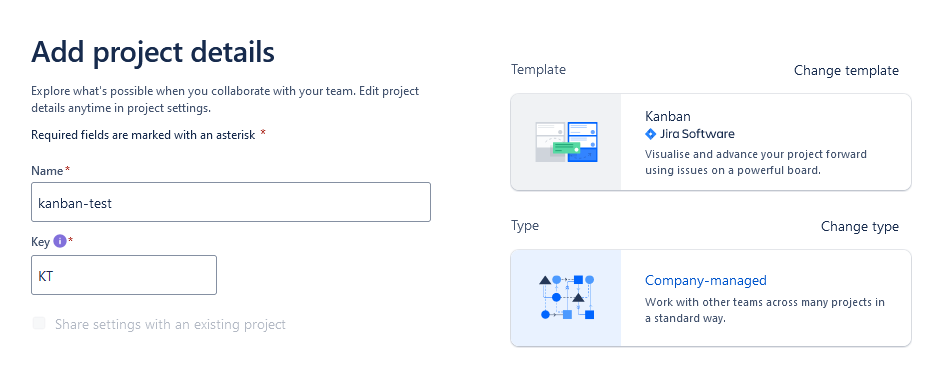
\includegraphics[width=15cm,keepaspectratio]{rysunki/jira-create-project.png}
    \caption{Tworzenie projektu Kanban w konfiguracji Company-managed}
\end{figure}

\begin{figure}[H]
    \centering
    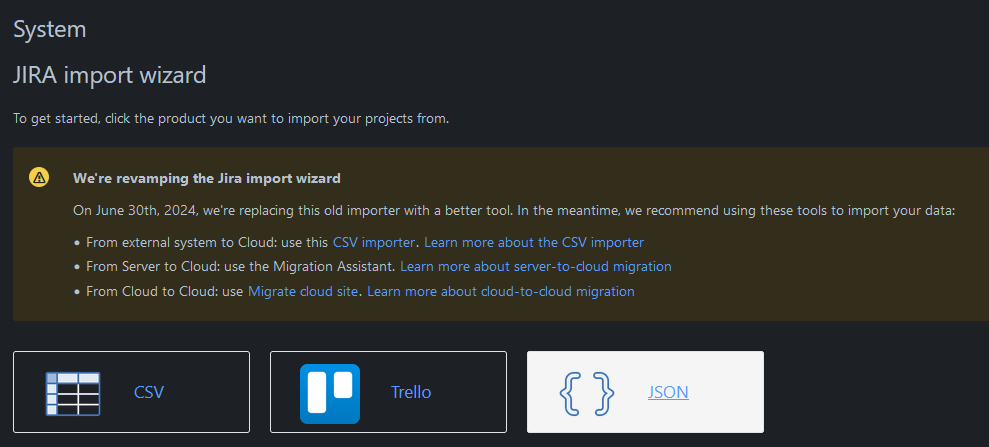
\includegraphics[width=15cm,keepaspectratio]{rysunki/jira-import-wizard.png}
    \caption{Narzędzie do importu danych na Jirę}
\end{figure}

Po pomyślnym zakończeniu importu danych, wszystkie zadania możemy zaobserwować w projekcie.
\begin{figure}[H]
    \centering
    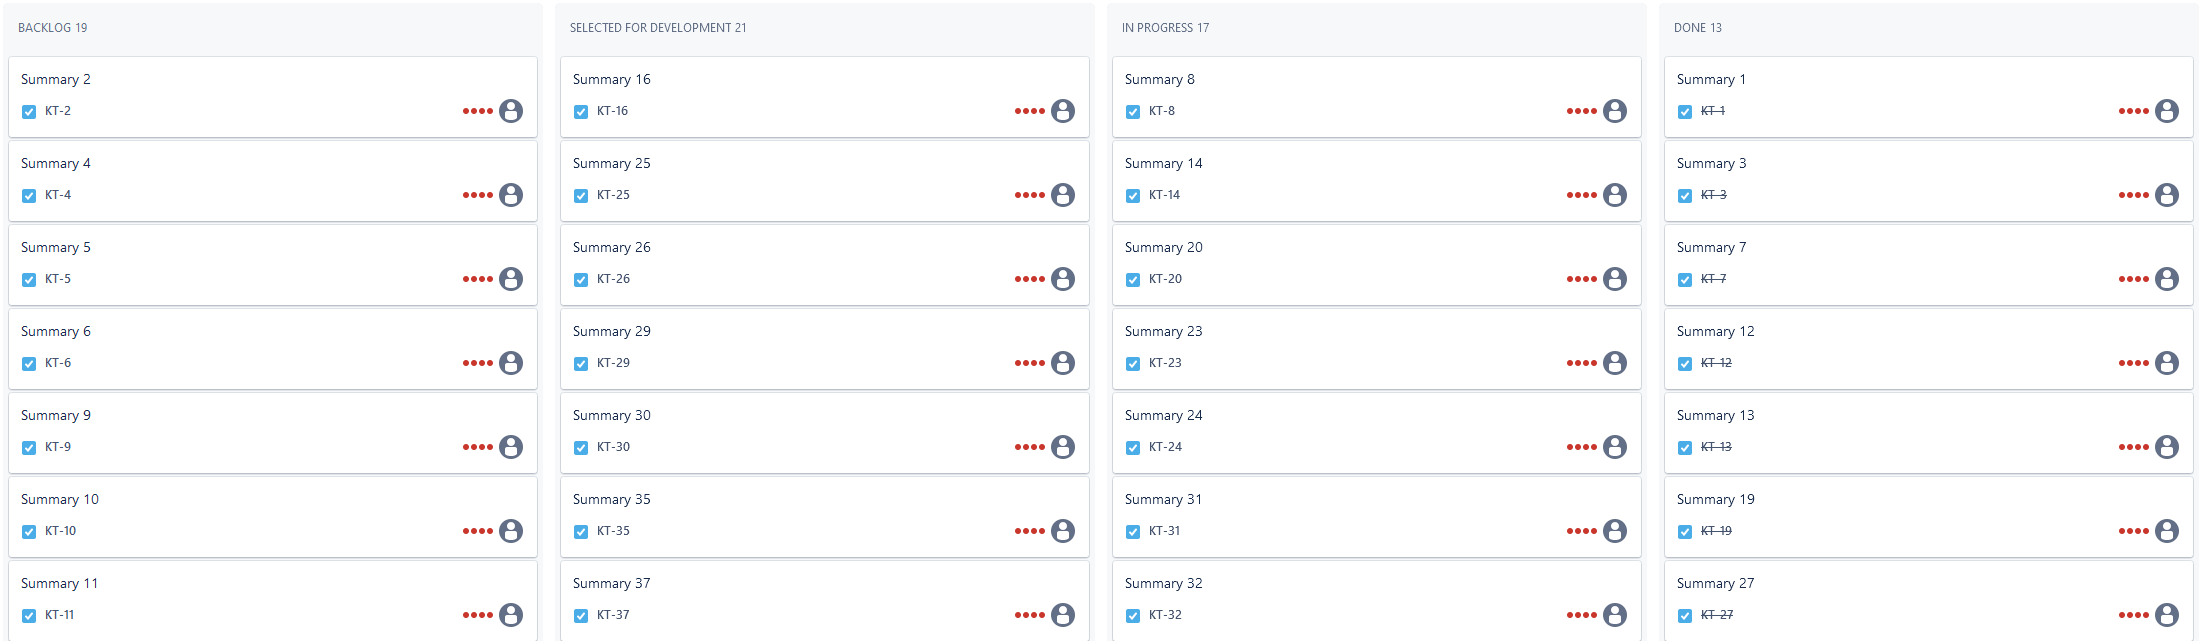
\includegraphics[width=15cm,keepaspectratio]{rysunki/jira-board.png}
    \caption{Fragement tablicy wypełnionej zaimportowanymi zadaniami}
\end{figure}

Przy inspekcji zakładki "History" w zadaniu możemy zaobserwować poprawną chronologię w zmianach statusów.
\begin{figure}[H]
    \centering
    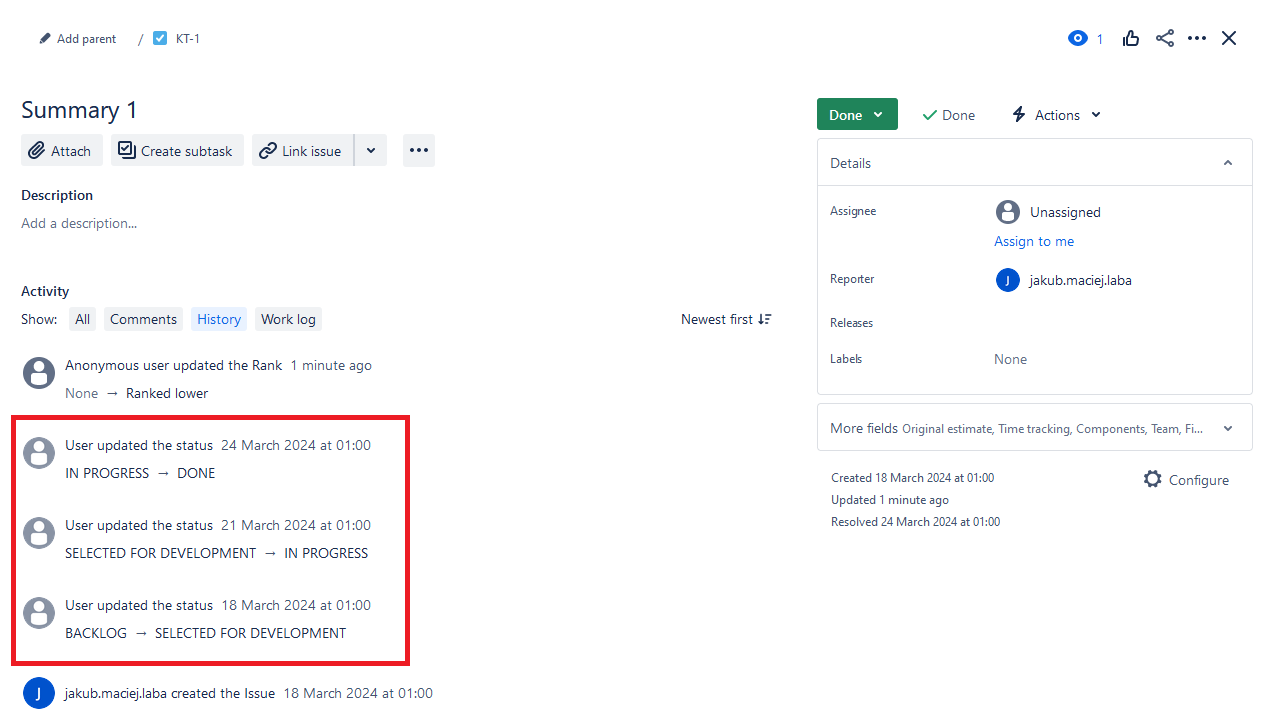
\includegraphics[width=15cm,keepaspectratio]{rysunki/jira-issue-history.png}
    \caption{Historia przykładowego zaimportowanego zadania}
\end{figure}

\section{Przykład analizy metryk}
Z uwagi na fakt, że zaimplementowanie integracji z wbudowanymi narzędziami analitycznymi nie było możliwe, niestety nie można przeprowadzić analizy metryk bezpośrednio na Jirze. Nadal można jednak łatwo wydobyć potrzebne
dane za pomocą JQL, a następnie obliczyć je w arkuszu kalkulacyjnym lub narzędziu do analizy biznesowej.

Ten podrozdział prezentuje przykładowe zapytania JQL, które można zastosować do wydobycia danych potrzebnych do analizy metryk.

\subsection{Wiek pracy w toku}
W celu obliczenia wieku pracy w toku dla konkretnego zadania, można wydobyć je prostym zapytaniem o klucz: \lstinline{key = "KT-3"}.
Następnie należy obliczyć ilość dni pomiędzy obecną datą, a datą utworzenia zadania.
Na podobnej zasadzie można obliczyć średni wiek pracy w toku dla większej ilości zadań dla celów monitorowania produktywności, aby szybko identyfikować blokujące się zadania gdy zaczynają znacznie przekraczać średnią wartość tej metryki.

\subsection{Przepustowość}
Przepustowość można otrzymać licząc ilość wyników zwróconych przez zapytanie JQL, filtrujące zadania po przejściu do wybranego statusu oznaczającego zakończenie zadania, oraz w wybranym przedziale czasowym.
\begin{lstlisting}[caption=Zapytanie JQL pozwalające obliczyć przepustowość w przeciągu ostatniego tygodnia]
status CHANGED TO "Done" DURING (-7d, now())
\end{lstlisting}

\subsection{Efektywność przepływu}
Do obliczenia efektywności przepływu potrzeba zidentyfikować które statusy były aktywne, a które pasywne.

W rozpatrywanym tutaj przypadku testowym, jedynym aktywny statusem był "In Progress", należy więc znaleźć wszystkie zadania które znajdowały się w tym statusie.
\begin{lstlisting}[caption=Zapytanie JQL pozwalające obliczyć efektywność przepływu]
status WAS "In Progress"
\end{lstlisting}

W otrzymanych wynikach wyszukiwania za pomocą wybranego narzędzia należy obliczyć całkowity czas znajdowania się w statusach aktywnych i pasywnych, oraz obliczyć proporcję jednego do drugiego.

\subsection{Czas realizacji}
Do obliczenia czasu realizacji potrzeba zdefiniować który status jest punktem realizacji, a który punktem dostarczenia.

W rozpatrywanym tutaj przypadku testowym, punktem zobowiązania był status "Selected for Development", natomiast punktem dostarczenia status "Done".
\begin{lstlisting}[caption=Zapytanie JQL pozwalające obliczyć czas dostarczenia w przeciągu ostatniego tygodnia]
status WAS "Selected for Development" DURING (-7d, now())
AND status CHANGED TO "Done" DURING(-7d, now())
\end{lstlisting}

Następnie w wybranym narzędziu należy obliczyć okres pomiędzy datami znalezienia się zadania w tych dwóch statusach.
Na podobnej zasadzie można obliczyć średni czas realizacji dla większej ilości zadań w celu zdobycia danych do estymacji jakie zobowiązania można podjąć wobec klienta.


\chapter{Podsumowanie}
Celem pracy "Generowanie danych na potrzeby nauki metryk w inżynierii oprogramowania" było stworzenie rozwiązania umożliwiającego symulację projektów z użyciem popularnych platform w kontrolowanym środowisku. Dzięki temu
zespoły oraz osoby uczące się mogłyby doskonalić umiejętność analizy i interpretacji metryk bez konieczności pracy w rzeczywistymi danymi, które mogą być poufne lub po prostu trudne do zdobycia. W rezultacie powstała aplikacja
w formie programu CLI, umożliwiająca generowanie danych do symulacji projektów prowadzonych w metodyce Kanban na platformie Jira.

Prace rozpoczęły się od analizy różnych metryk stosowanych stosowanych do pomiaru efektywności zespołów w kontekście inżynierii oprogramowania. Przeprowadzony został również przegląd platform do zarządzania projektami, ze szczególnym
uwzględnieniem Jiry i YouTracka, skupiając się na metrykach związanych z metodyką Kanban.

Kolejnym krokiem była analiza struktury danych projektów i zadań, opierając się na dokumentacji oraz technikach reverse-engineering. To pozwoliło na zdefiniowanie podstawowych mechanizmów, kluczowych dla implementacji rozwiązania.

Aplikacja agilemaster pozwala na szybkie generowanie danych projektowych przy minimalnej konfiguracji. Aplikacja umożliwia wybór okna czasowego w którym mają być generowane zadania oraz wprowadzenie dowolnych statusów zadań, co pozwala
na elastyczność pod kątem scenariuszy lub wymagań projektów tworzonych z różnych szablonów lub według niestandardowych spersonalizowanych konfiguracji.

Rozwiązanie może być niezwykle wartościowe dla celów szkoleniowych, ponieważ umożliwia naukę w środowisku, które jest zgodne z rzeczywistymi warunkami komercyjnymi. Osoby uczące się analizy metryk i zarządzania projektami w metodykach
zwinnych mogą teraz ćwiczyć i eksperymentować z różnymi scenariuszami, zyskując cenne doświadczenie.

Poprzez dostarczenie praktycznego narzędzia, znacznie usprawniającego proces nauki analizy metryk, praca może przyczynić się do popularyzacji wiedzy niosącej za sobą znaczącą wartość biznesową.


\chapter{Możliwości dalszego rozwoju projektu}
W obecnej formie aplikacja posiada jedynie podstawowe funkcjonalności, pozostawiając nadal wiele pola do rozwoju.

Istotnym ulepszeniem byłaby wspomniana integracja z narzędziami do generowania wykresów wbudowanymi bezpośrednio w Jirę aby zwiększyć wygodę analizy generowanych danych.

Wiele wartości dodałaby tutaj możliwość dokładniejszej kontroli nad parametrami generowania, aby móc tworzyć bardziej precyzyjne scenariusze do nauki, pozwalając np. na celowe generowanie projektów
które postępują bardzo sprawnie lub wręcz przeciwnie. Do osiągnięcia takich rezultatów można by było wprowadzić kontrolę nad rozkładem zadań w różnych statusach -- konfigurując precyzyjne ilości lub
ich proporcje do siebie nawzajem. Innym parametrem którego kontrolowanie pozwoliłoby zwiększyć atrakcyjność aplikacji jest możliwość manipulacji czasem trwania zadań lub czas ich przebywania w 
poszczególnych statusach -- w sposób precyzjny, lub na podstawie wybranych rozkładów losowych.

Jeśli chodzi o kompatybilność aplikacji z więcej niż jedną platformą, jest to poniekąd osiągnięte poprzez wybór Jiry, będącej najpopularniejszą z nich.
Popularnością Jiry podyktowana jest możliwość importu projektów z niej w innych narzędziach, takich jak YouTrack czy Azure DevOps.
